%!TEX root = brochistochrone.tex


\section{역사적 단상}

\begin{itemize}
\item 갈릴레오; (중심각이 $90^\circ$인) 원호 모양의 철사에 구슬을 꿰었을 때, 마찰없이 구슬이 미끄러지는데 걸리는 시간을 생각하였다. 
\begin{center}
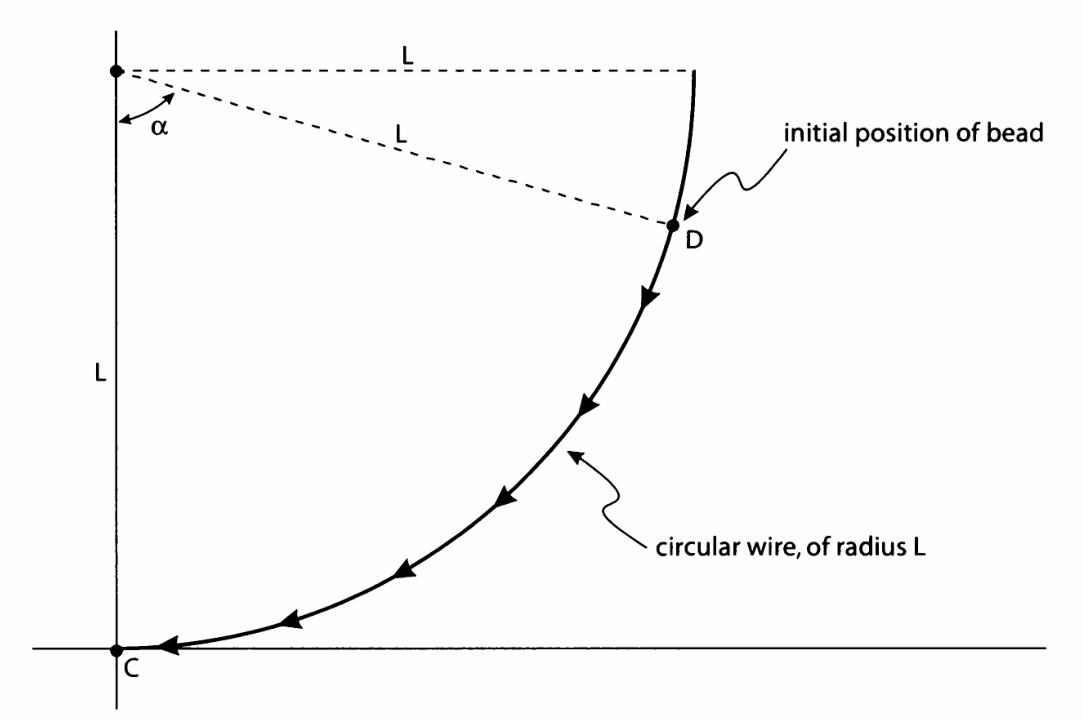
\includegraphics[width=.7\textwidth]{images/gal01}
\end{center}
미적분의 이론을 통해 구슬의 강하시간을 계산하면 
\[
\sqrt{\frac{L}{g}}\int_0^{\pi/2}\frac{1}{\sqrt{1-\sin^2\left(\frac{1}{2}\alpha\right)\sin^2\beta}}\ \mathrm{d}\beta
\]
이고, 이는 약 $1.8541\sqrt{L/g}$이다.

\item 갈릴레오는 원호를 다각선으로 근사시켰을 때의 낙하시간이 항상 원호를 따를 때의 낙하시간보다 크다고 추론하였다.\footnote{자세한 내용이 참고도서 \cite{PaulNahin}의 6.1절에 소개되어있다.} 어떤 사람들은 갈릴레오가 최단강하선이 원호임을 주장했다고 하는데, 이는 역사학자들 사이에 여러 이견이 있는 듯 하다.  
\item 요한 베르누이는 1696년 학술지 Acta Eruditorum에서 ``세계에서 가장 뛰어난 수학자들(the most brilliant mathematicians in the world)''을 향해 다음과 같은 문제를 제시하였다.\footnote{1682년에 처음으로 출판된 독일 최초의 학술지.}
\begin{quote}
``어떤 물체가 점 $\mathrm{A}$에서 출발하여 점 $\mathrm{B}$까지 중력에 의해서만 이동할 때, 소요시간을 최소화하려면 이 물체는 어떤 경로를 따라 이동해야하는가?''
\end{quote}
이 문제에 대해, 야곱 베르누이, 라이프니츠, 로피탈 등 여러 수학자가 옳은 답을 제시하였다. 그리고 익명으로 투고된 답안도 있었다. 요한은 이 답안을 보고 ``발톱 자국으로부터 그것이 사자의 것임을 알 수 있다.''라고 말했다고 한다.\cite{Wiki}
\item 베르누이의 도전은 결코 호의적이지 않았다. 그리고 베르누이는 갈릴레오의 업적은 전혀 언급하지 않았으며, 오히려 최단강하에 관해 갈릴레오의 업적은 전혀 알지 못했었다고 주장했다. 또한 베르누이는 뉴턴과 사이가 좋지 못했는데, 이 최단강하선의 풀이에 대한 찬사가, 뉴턴을 향한 거의 유일한 좋은 평가라고 한다.\cite{PaulNahin} 사실 요한 베르누이는 미적분학의 창시자가 누구인가에 대한 싸움에서 라이프니츠의 편에서서 전투적인 모습을 보였었다고 한다.\cite{William}
\end{itemize}

\section{준비학습: 에너지 보존법칙}

\begin{itemize}
\item 질량이 $m$인 물체가 $v=y'(t)$의 속도로 자유낙하하고 있을 때, 이 물체의 운동에너지는 $\frac{1}{2}mv^2=\frac{1}{2}m(y'(t))^2$으로 정의되며, 이 물체의 위치에너지는 $mgy(t)$로 정의된다. 그리고 운동에너지와 위치에너지의 합을 역학적 에너지라고 한다.

\item 중력에 의해서 자유낙하하는 물체의 가속도는 $y''(t)=-g$이다. 역학적 에너지를 시간 $t$에 대하여 미분해보면
\begin{align*}
\frac{\mathrm{d}}{\mathrm{d}t}\left( \frac{1}{2}m(y'(t))^2+mgy(t)\right) &= my'(t)y''(t)+mgy'(t) \\
&= -mgy'(t)+mgy'(t)=0
\end{align*}
임을 알 수 있다. 따라서 역학적 에너지의 총량은 시간에 따라 변하지 않음을 알 수 있다.

\item 중력장 안에서 $3$차원 운동을 하고 있는 질량 $m$인 물체의 시각 \(t\)에서의 위치를 $\mathbf{X}(t)=(x(t), y(t), z(t))$라 하면, 이 물체의 운동에너지는
\[
\frac{1}{2}m\Vert \mathbf{X}'(t)\Vert^2,
\]
위치에너지는
\[
mgz(t)
\]
이다. 중력에 의해서만 운동하는 이 물체의 역학적 에너지를 시간에 대해 미분해보면
\begin{align*}
\frac{\mathrm{d}}{\mathrm{d}t}\left( \frac{1}{2}m\Vert \mathbf{X}'(t)\Vert^2+mgz(t)\right)& = \frac{\mathrm{d}}{\mathrm{d}t}\left( \frac{1}{2}m(\mathbf{X}'(t)\bullet\mathbf{X}'(t))+mgz(t)\right) \\
& = m (\mathbf{X}'(t)\bullet\mathbf{X}''(t))+mgz'(t) \\
& = m\left( (x'(t), y'(t), z'(t))\bullet(0, 0, -g)\right)+mgz'(t) \\
&= -mgz'(t)+mgz'(t)=0
\end{align*}
으로 역시 역학적 에너지는 시간에 따라 변하지 않음을 알 수 있다.
\item 물체의 운동을 살펴볼 때, 물체가 가진 속도, 에너지 등 물리적인 정보를 해석하기 위해서는 그 물체에 작용하는 모든 힘을 고려해야한다. 지금 살펴보고 있는 운동에서는
\begin{enumerate}[(a)]
\item 마찰력이나 공기의 저항은 무시하고 있다.
\item 중력의 영향을 고려하고 있다.
\item 철사 혹은 미끄럼틀 같은 경로를 정해주어 물체의 이동에 영향을 주고 있다.
\end{enumerate}
정도를 생각해볼 수 있다. 그런데, 물체가 가진 에너지에 대해서는 (c)의 영향을 고려하지 않아도 된다. 왜냐하면, 소위 `구속된 운동'에서의 구속력은 늘 물체의 이동방향에 수직으로 작용하므로 그 구속력이 하는 일은 늘 $0$이기 때문이다.
\end{itemize}

\section{베르누이의 풀이}

스넬의 법칙을 상기해보자. 그림과 같이 서로 다른 매질1, 매질2가 있고 각각을 통과할 때의 속력이 $v_1, v_2$라고 할 때, B에서 A로 가는 빛의 경로는 
\[
\frac{\sin\theta_1}{v_1}=\frac{\sin\theta_2}{v_2}
\]
를 만족시킨다. 최단 강하선 문제에 대한 요한 베르누이의 풀이는 에너지 보존 법칙과 스넬의 법칙을 이용한 풀이이다.

\begin{center}
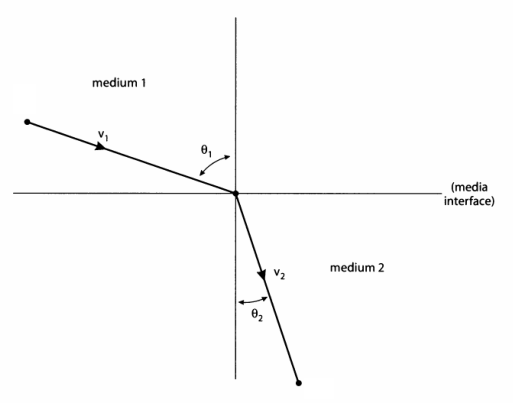
\includegraphics[width=.8\textwidth]{images/snellslaw}
\end{center}

이제 베르누이의 풀이를 살펴보자. 먼저 최단 강하선 $y=f(x)$가 있을 때, 이 곡선이 만족시켜야 하는 조건이 무엇인지 살펴보자. 편의상 $y$축의 방향을 아래쪽으로 향하게 하고\footnote{즉 $y$축의 방향을 속력이 증가하는 방향으로 두고} 점 $\mathrm{A}$를 원점에 위치시키자. 그리고 점 $\mathrm{B}$의 좌표는 $(b_1, b_2)$로 쓰자.  그림과 같이 $y$축을 $n$등분하는 가로선들을 그어, 이 가로선이 최단강하선과 만나는 점들을 $\mathrm{P}_i(x_i, y_i), i=1,\ldots, n$로 쓰자.   물론 $\mathrm{A}=\mathrm{P}_0, \mathrm{B}=\mathrm{P}_n$이다.

\begin{center}
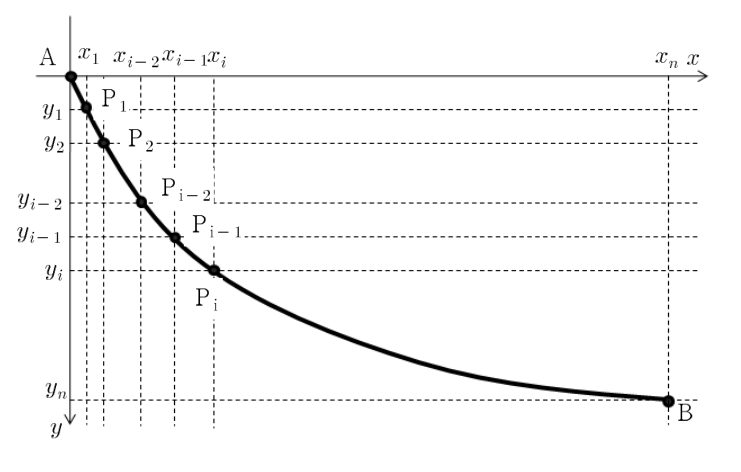
\includegraphics[width=.9\textwidth]{images/bernsol01}
\end{center}

베르누이는 위 그림에서의 가로선들을 서로 다른 매질들의 경계면으로 생각하였다. 즉 최단강하선의 문제를 아래로 갈수록 덜 조밀한(즉 아래로 갈 수록 빛이 더 빠르게 이동할 수 있는) 여러개의 층이 있을 때, 빛이 어떻게 이동하는가에 대한 문제를 통해 살펴본 것이다.

\begin{center}
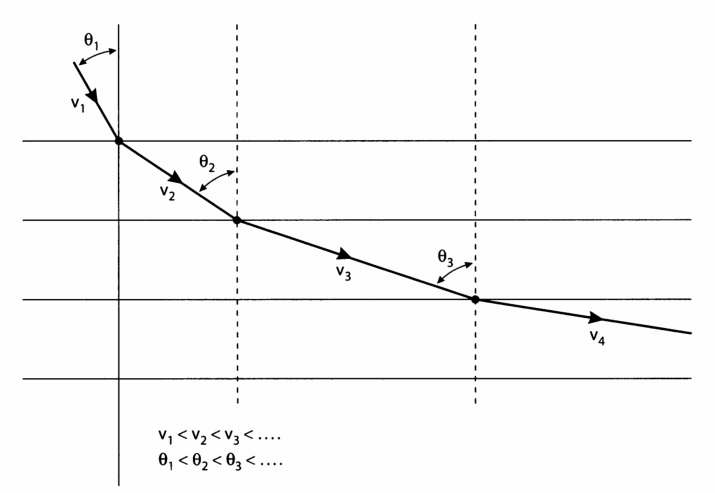
\includegraphics[width=.8\textwidth]{images/bernsol02}
\end{center}

그림의 경로가 빛의 경로, 즉 소요시간을 최소화하는 경로라면, 역시 스넬의 법칙에 따라 모든 $i$에 대하여
\[
\frac{\sin\theta_{i-1}}{v_{i-1}}=\frac{\sin\theta_i}{v_i}
\]
가 성립한다. 따라서
\[
\frac{\sin\theta_i}{v_i}=\mbox{(상수)}
\]
로 둘 수 있다. 이제  층의 개수를 무한히 증가시키면 빛의 경로는 부드러운 곡선을 따르게 되는데, 그림과 같이 각 점에서의 속력 $v$에 대하여 등식
\begin{equation}\label{eq:snellslaw}
\frac{\sin\theta}{v}=\mbox{(상수)}
\end{equation}
가 성립한다.

\begin{center}
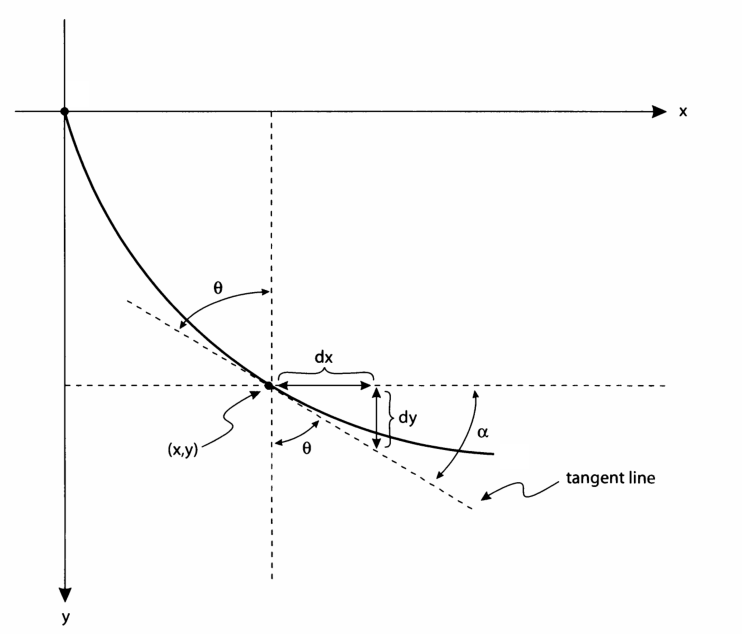
\includegraphics[width=.7\textwidth]{images/bernsol03}
\end{center}

이때 점 $\mathrm{P}(x, y)$에서의 속력 $v$는 에너지 보존 법칙을 이용해 구할 수 있다. 에너지 보존 법칙에 따르면, 물체가 낙하하면서 줄어든 위치 에너지만큼 그 물체가 가진 운동에너지가 증가한다. 그런데 %점 $\mathrm{P}_i$에서의 속력 $v_i$를 구할 수 있다. %위와 같이 좌표를 설정해두었으면 
점 $\mathrm{P}(x, y)$에서 처음에 비해 줄어든 위치에너지는 $mgy$이고 $\mathrm{P}_0$에서 이 물체가 가진 운동에너지가 $0$이었으므로 늘어난 운동 에너지는 $\frac{1}{2}mv^2$이고 이는  $mgy$와 같다. 따라서
\begin{equation}\label{eq:energy}
v=\sqrt{2gy}
\end{equation}
가 성립한다. 위의 그림에서와 같이 접선이 가로선과 이루는 각을 $\alpha$라 하면, $\theta+\alpha=\pi/2$이고 따라서
\begin{align*}
\sin\theta&=\cos\alpha=\frac{1}{\sec\alpha}=\frac{1}{\sqrt{1+\tan^2\alpha}} \\
& = \frac{1}{\sqrt{1+(\mathrm{d}y/\mathrm{d}x)^2})}=\frac{1}{\sqrt{1+(y')^2}}
\end{align*}
이 성립한다. 이 결과와 식 \eqref{eq:snellslaw}\와 \eqref{eq:energy}\를 이용하여
\[
(\mbox{상수})=\frac{\sin\theta}{v}=\frac{\frac{1}{\sqrt{1+(y')^2}}}{\sqrt{2gy}}=\frac{1}{\sqrt{2gy}\sqrt{1+(y')^2}}
\]
을 얻는다. 이로부터 최단 강하선이 만족시키는 미분방정식
\begin{equation}\label{eq:diffeq}
y(1+(y')^2)=C%_{\text{상수}}
\end{equation}
를 얻는다.\par 


일반적으로 선형이 아닌 미분방정식은 해를 구하는 것이 쉽지는 않지만, 식 \eqref{eq:diffeq}\는 변수분리형 미분방정식으로 해를 구할 수 있다. 실제로 식 \eqref{eq:diffeq}\를
\[
\mathrm{d}x=\mathrm{d}y\sqrt{\frac{y}{C-y}}
\]
로 변형하고, $\tan\varphi=\sqrt{\frac{y}{C-y}}$로  두면
\begin{align*}
&\frac{y}{C-y}=\tan^2\varphi=\frac{\sin^2\varphi}{\cos^2\varphi}\\
\Rightarrow\quad & y\cos^2\varphi =C\sin^2\varphi -y\sin^2\varphi \\
\Rightarrow\quad & y=C\sin^2\varphi 
\end{align*}
를 얻는다. 이제 $x$를 매개변수 $\varphi$로 나타낼 수 있으면, 곡선 $y=f(x)$의 매개변수 표현을 얻는 것이 된다. 위의 마지막 식을 미분하여 $\mathrm{d}y=2C\sin\varphi\cos\varphi\ \mathrm{d}\varphi$를 얻고 이를 이용해
\begin{align*}
\mathrm{d}x&=\mathrm{d}y\sqrt{\frac{y}{C-y}}=2C\sin\varphi\cos\varphi\tan\varphi\ \mathrm{d}\varphi \\
&= 2C\sin^2\varphi\ \mathrm{d}\varphi \\
&= C(1-\cos(2\varphi))\ \mathrm{d}\varphi
\end{align*}
즉 $\mathrm{d}x=C(1-\cos(2\varphi))\ \mathrm{d}\varphi$를 얻고, 양변을 적분하여 $x=\frac{1}{2} C(2\varphi-\sin(2\varphi))+C_0$를 얻는다. 여기서 적분상수 $C_0$는 초기조건을 통해 $0$임을 바로 알 수 있다. 이제 $2\varphi=\theta, R=\frac{1}{2}C$로 두면 곡선 $y=f(x)$의 매개변수 표현
\[
x=R(\theta-\sin\theta),\quad y=%C\sin^2\varphi=\frac{1}{2}C(1-\cos(2\varphi))=
R(1-\cos\theta)
\]
를 얻는다. 이는 그 유명한 사이클로이드 곡선의 매개변수 표현이다.

\begin{itemize}
\item 상수 $R$을 적절히 조절하면, 임의의 점 $(x, y)$ (단, $x>0, y>0$)를 지나는 사이클로이드를 정할 수 있다.

\item 베르누이의 풀이를 다시 살펴보면, 다음의 두 가지 가정을 중요한 역할을 하고 있음을 알 수 있다. 그리고 이 가정들은 타당하다고 생각된다.
\begin{itemize}
\item  곡선 $ y=f(x)$를 각 $\mathrm{P}_i$를 잇는 선분 경로들의 모임으로 근사시켜서 생각한다. %그리고 $n$이 충분히 클 때, 이는 실제 물체의 운동에 대한 좋은 근사가 된다.
\item  물체가 $\mathrm{P}_{i-1}$에서 $\mathrm{P}_i$까지 직선경로를 따르며 이동하는 속력이 $v_i$로 일정하다고 가정한다. 
\end{itemize}
\end{itemize}

\section{오일러-라그랑지 방정식과 변분법}

점 $\mathrm{P}_{i-1}$에서 $\mathrm{P}_i$까지 ($v_i$의 속력으로) 이동하며 걸리는 시간을 $T_{i-1}^i$라 하면, 최단강하선 문제는
\[
\lim_{n\to\infty}\sum_{i=1}^{n}T_{i-1}^i
\]
를 최소화 하는 것이다. 특히 $T_{i-1}^i=\frac{\overline{\mathrm{P}_{i-1}\mathrm{P}_i}}{v_i}$이므로 위 식을 다시 쓰면
\begin{align*}
\lim_{n\to\infty}\sum_{i=1}^{n}T_{i-1}^i&=\lim_{n\to\infty}\sum_{k=1}^n \frac{\sqrt{\Delta x_i^2+\Delta y_i^2}}{v_i} \\
& = \lim_{n\to\infty}\sum_{i=1}^n \frac{\sqrt{1+(\Delta y_i/\Delta x_i)^2}}{\sqrt{2gy_i}}\cdot \Delta x_i
\end{align*}
이다. 즉 최단강하선 문제는
\[
\int_0^{b_1}\frac{\sqrt{1+(y')^2}}{\sqrt{2gy}} \mathrm{d}x
\]
를 최소화하는 문제이다.  다시 말해, 
\begin{quote}
``주어진 경로에 따르는 소요시간을 재는 함수 $T$를 생각할 때, $T$가 최소가 되는 $y=f(x)$가 무엇인가?''
\end{quote}
가 궁금한 것이다. 여기서 $T$는 곡선(함수)을 실수로 대응시키는 범함수이다. 이처럼 범함수의 극대, 극소(혹은 최대, 최소)를 찾는 기법을 변분법이라고 부른다. \par 

미분가능한 함수  $f:[0, b_1]\to\mathbb{R}$와 이변수 함수 $\mathscr{L}(u, v):=\frac{\sqrt{1+v^2}}{\sqrt{2gu}}$를 생각할 때, 이를 이용하여 얻은 범함수
\[
T(f)=\int_0^{b_1}\mathscr{L}(f(x), f'(x)) \mathrm{d}x% =\int_0^{b_1}\frac{\sqrt{1+(f'(x))^2}}{\sqrt{2gf(x)}} \mathrm{d}x
\]
의 최솟값을 생각하는 것이 바로 최단강하선 문제이다.\par 

$T$는  함수들의 집합 $\mathscr{F}=\{ f\in C^\infty[0, b_1]\mid f(0)=0, f(b_1)=b_2\} $에서 정의된 범함수이다. 만일 $f$가 $T$를 최소가 되게 하는 함수라면, 임계점 정리에 의해, 임의의 함수
\[
h:[0, b_1]\to \mathbb{R},\quad h(0)=0, h(b_1)=0 
\]
에 대하여, 
\[
g(t):=\int_0^{b_1}\mathscr{L}(f(x)+th(x), f'(x)+th'(x)) \mathrm{d}x
\]
는 $t=0$에서 최솟값을 갖는다. 따라서
\begin{align*}
0=g'(t)&= \frac{\mathrm{d}}{\mathrm{d}t}\Big\vert_{t=0} \int_0^{b_1}\mathscr{L}(f(x)+th(x), f'(x)+th'(x)) \mathrm{d}x \\
&= \int_0^{b_1} \frac{\mathrm{d}}{\mathrm{d}t}\Big\vert_{t=0} \mathscr{L}(f(x)+th(x), f'(x)+th'(x)) \mathrm{d}x \\
&= \int_0^{b_1} \frac{\partial}{\partial u}\mathscr{L}(f(x), f'(x) )\cdot h(x)+\frac{\partial}{\partial v}\mathscr{L}(f(x), f'(x))\cdot h'(x)\ \mathrm{d}x \\
&= \int_0^{b_1}\left( \frac{\partial}{\partial u}\mathscr{L}(f(x), f'(x))-\frac{\mathrm{d}}{\mathrm{d} x}\frac{\partial}{\partial v}\mathscr{L}(f(x), f'(x))\right)h(x)\ \mathrm{d}x
\end{align*}
가 성립한다. 여기서 $h$는 임의의 함수이므로 방정식
\begin{equation}\label{eq:eulerlagrange}
\frac{\partial}{\partial u}\mathscr{L}(f(x), f'(x))=\frac{\mathrm{d}}{\mathrm{d} x} \frac{\partial}{\partial v}\mathscr{L}(f(x), f'(x))
\end{equation}
를 얻는다.  $T$의 극값이 되는 함수 $y=f(x)$는 방정식 \eqref{eq:eulerlagrange}\를 만족시켜야 한다. 방정식 \eqref{eq:eulerlagrange}\를 오일러-라그랑지 방정식이라 부른다. \par 

오일러-라그랑지 방정식의 양변에 $f'(x)$를 곱하면
\[
f'(x) \frac{\partial}{\partial u}\mathscr{L}(f(x), f'(x))=f'(x) \frac{\mathrm{d}}{\mathrm{d} x} \frac{\partial}{\partial v}\mathscr{L}(f(x), f'(x))
\]
이고, 이 식에 다시 $f''(x)\frac{\mathrm{\partial}}{\partial v}\mathscr{L}(f(x), f'(x))$를 더하여
\begin{align*}
f'(x) \frac{\partial}{\partial u}\mathscr{L}(f(x), f'(x)) +& f''(x)\frac{\mathrm{\partial}}{\partial v}\mathscr{L}(f(x), f'(x)) \\
&=f'(x) \frac{\mathrm{d}}{\mathrm{d} x} \frac{\partial}{\partial v}\mathscr{L}(f(x), f'(x))+f''(x)\frac{\mathrm{\partial}}{\partial v}\mathscr{L}(f(x), f'(x))
\end{align*}
를 얻는데, 이를 다시 쓰면
\[
\frac{\mathrm{d}}{\mathrm{d}x}\mathscr{L}(f(x), f'(x))=\frac{\mathrm{d}}{\mathrm{d}x}\left( f'(x) \frac{\partial}{\partial v}\mathscr{L}(f(x), f'(x))\right)
\]
이다. 따라서
\begin{equation}\label{eq:soleq}
\mathscr{L}(f(x), f'(x))=f'(x)\frac{\partial}{\partial v}\mathscr{L}(f(x), f'(x))+C
\end{equation}
를 얻는다. 특히 $\mathscr{L}(u, v)=\frac{\sqrt{1+v^2}}{\sqrt{2gu}}$이므로 $\frac{\partial}{\partial v}\mathscr{L}(u, v)=\frac{v}{\sqrt{2gu}\sqrt{1+v^2}}$이고 이를 식 \eqref{eq:soleq}에 대입하여
\[
\frac{\sqrt{1+(f'(x))^2}}{\sqrt{2gf(x)}}=f'(x)\cdot \frac{f'(x)}{\sqrt{2gf(x)}\sqrt{1+(f'(x))^2}}+C
\]
를 얻는다. 이 식을 정리하면 베르누이의 풀이에서 얻은 것과 동일한 미분방정식인
\[
y(1+(y')^2)=\text{Const.}
\]
를 얻는다.

\section{추가 질문}

\begin{itemize}
\item 최단 강하선의 문제의 해는 유일한가?%; 미분방정식 관련 글을 찾아보니, 해석적인 해는 유일하다는 것 같다.
\item 거슬러 올라갈 수 없다는 조건이 추가된다면 어떤 경로를 택해야 할까?%; 몇 가지 경로를 생각하여 비교를 해봐야 할 것이다.
\item 원호, 직선 경로의 경우에서의 소요시간과 사이클로이드의 소요시간을 비교해보면 어떠한가?%; 구체적으로 식을 세울 수 있다. 그러나 원호의 경우 소요시간을 닫힌형태로 쓸 수 없는 타원적분으로 표현된다.
\end{itemize}

\begin{thebibliography}{99}
\bibitem{amg-lecturenote} 윤종국, \emph{현대기하학 강의록(최소 하강선과 변분법)}
\bibitem{PaulNahin}  Paul J.\ Nahin,
\emph{When Least is Best},
Princeton University Press, (2004) / 번역서 있음: `최상의 최소(경문사/권오남 외 번역)'
\bibitem{KimHJ} 김홍종,  
\emph{미적분학2+},
서울대학교 출판부, (2017)
\bibitem{William} William Dunham, 
\emph{The Calculus Gallery},
Princeton University Press, (2005) / 번역서 있음: `미적분학 갤러리(청문각/권혜승 번역)'
\bibitem{Wiki} Wikipedia,
\href{https://en.wikipedia.org/wiki/Brachistochrone_curve}{\emph{https://en.wikipedia.org/wiki/Brachistochrone\_curve}}
%\bibitem{WikiActa} Wikipedia, \href{https://en.wikipedia.org/wiki/Acta_Eruditorum}{\emph{https://en.wikipedia.org/wiki/Acta\_Eruditorum}}
\end{thebibliography}
